% Chapter 4

\chapter{Internship Subject} % Main chapter title

\label{Chapter3} % For referencing the chapter elsewhere, use \ref{Chapter3}

%----------------------------------------------------------------------------------------

% Define some commands to keep the formatting separated from the content
%\newcommand{\keyword}[1]{\textbf{#1}}
%\newcommand{\tabhead}[1]{\textbf{#1}}
%\newcommand{\code}[1]{\texttt{#1}}
%\newcommand{\file}[1]{\texttt{\bfseries#1}}
%\newcommand{\option}[1]{\texttt{\itshape#1}}

%----------------------------------------------------------------------------------------

\section{Problematics}

As I said in the previous parts, \iBubble{} includes a visual tracking system, \keyword{CMT}, to \emph{autonomously} follow divers underwater. This system currently uses \emph{openCV} libraries at a rate of \textbf{30 fps}. This speed can be improved using \emph{CUDA} technology. These features are only available on \keyword{BtB} versions of \iBubble{} fitted with \emph{Nvidia's Jetson embedded board}.

\keyword{BtC} versions of the drone uses \rasp{} in spite of the current \emph{Nvidia Graphics Card} wich means that \emph{CUDA} is no longer available because \vc{} is not designed with this technology.

As a consequence, \vc{} is not used so the whole tracking system is running only on the \cpu{} and the system rate drops to \textbf{7 fps}.

The more time-consuming part of the \keyword{CMT} is the \keyword{optical flow} computation. This is a fundamental tracking algorithm in Computer Vision. It uses \keyword{Gradient Descent} and \keyword{Pyramid} algorithms to get the displacement of the points of interest between two frames.

Therefore if we want to use the computing power of the \vc{}, it is compulsory to make our own implementation of the \keyword{optical flow} on \rasp, that was my internship subject.

The main difficulty is that there is no official \keyword{API} released by \textsc{Broadcom}. To compute the \keyword{optical flow} on \rasp, it was to necessary to follow the same steps as in Chapter~\ref{Chapter2}, namely:
\begin{itemize}
	\item write \code{code-to-execute} on \keyword{GPU} -- in \option{assembly language}
	\item parse this \code{code-to-execute} with \keyword{assembly parser} -- \file{qpu-asm.cpp}
	\item write a \code{driver program} for the \keyword{CPU} -- in \option{c-language}
	\item include this \keyword{API} in a \option{C++} project -- \keyword{CMT} is written in \option{C++}
\end{itemize}

%----------------------------------------------------------------------------------------

\section{Optical Flow}

Within \iBubble{} visual tracking system - \keyword{CMT} - \keyword{optical flow} is the displacement of points of interest - called \keyword{features} - between two consecutive frames from a video.

Computing \emph{optical flow} between two consecutive frames involves the following steps:
\begin{itemize}
	\item detect \keyword{features} on first image -- Figure~\ref{initFeaturesFig}
	\item find the next \keyword{features} positions on the second image -- Figure~\ref{secondFeaturesFig}
	\item compute \emph{displacemnt} for each \keyword{features} -- Figure~\ref{opticalFlowFig}
\end{itemize}


\begin{figure}[!htbp]
	\centering
	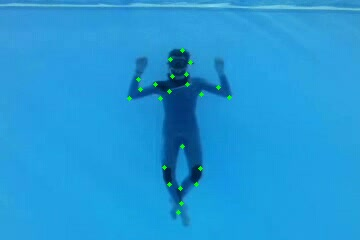
\includegraphics[width=0.5\textwidth]{plongeurInitFeatures}
	\caption{First frame of a diving video with the initial set of features}
	\label{initFeaturesFig}
\end{figure}
\FloatBarrier



\begin{figure}[!htbp]
	\centering
	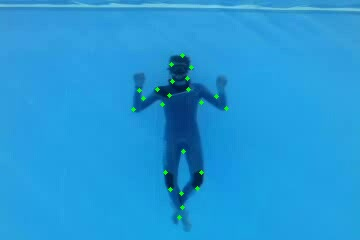
\includegraphics[width=0.5\textwidth]{plongeurNextFeatures}
	\caption{Second frame of a diving video with new features positions}
	\label{secondFeaturesFig}
\end{figure}
\FloatBarrier



\begin{figure}[!htbp]
	\centering
	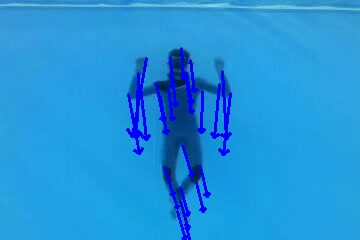
\includegraphics[width=0.5\textwidth]{plongeurOpticalFlow}
	\caption{Optical flow for the initial set of features -- \small{norm of the \textcolor{blue}{blue} vectors is overstated for better visualization}}
	\label{opticalFlowFig}
\end{figure}
\FloatBarrier

\emph{Optical flow} can be viewed as a \emph{vector field} representing \keyword{features} displacement between two consecutive frames. It is used to do object recognition, tracking or movement detection. In \iBubble, \emph{optical flow} is compute within \keyword{CMT} to achieve diver \emph{autonomous tracking and following}.\par

%----------------------------------------------------------------------------------------

\section{Lucas-Kanade method}

There are several ways to compute \keyword{optical flow}. Camille selected \keyword{Lucas-Kanade} method to be implemented on \vc.

The \emph{vision tracking} algorithm detects \keyword{30 features} on each frame from the camera. Thus, our \emph{homemade} algorithm must compute \keyword{optical flow} for these 30 features between two consecutive frames.


\subsection{Images encoding}

As I mentioned in~\ref{Matrices}, frames from the \rasp's camera (Figures~\ref{initFeaturesFig} to ~\ref{opticalFlowFig}) are \option{row major float-matrices}. More specifically, ($240\times 360$) pixel array:

\begin{figure}[!htbp]
\[
\begin{bmatrix}

pixel_{0,0} & pixel_{0,1} & \ldots & \ldots & \ldots & pixel_{0,359}\\

pixel_{1,0} & \ddots & \ldots & \ldots & \ldots & pixel_{1,359}\\

\vdots & \ldots & \ddots & \ldots & \ldots & \vdots\\

\vdots & \ldots & \ldots & feature_{x,y} & \ldots & \vdots\\

\vdots & \ldots & \ldots & \ldots & \ddots & \vdots\\

pixel_{239,0} & \ldots & \ldots  & \ldots & \ldots & pixel_{239,359}

\end{bmatrix}_{240\times 360}
\]
\caption{Frame from camera: two-dimensionnal pixel array}
\label{frameFig}
\end{figure}
\FloatBarrier

Moreover, \keyword{optical flow} algorithm uses \emph{grayscale} images:

\begin{itemize}
	\item each $pixel_{x,y}$ is encoded as \option{32-bit float}
	\item stored at @$pixel_{x,y}$ address
	\item @$pixel_{x,y}$ is a \option{32-bit integer} -- Appendice~\ref{AppendixB}
\end{itemize}\\~\\


From the shared RAM point of view, a frame is a contiguous array:
\begin{center}
\begin{tabular}{|c|c|c|}

	\hline
	\begin{bf}$\text{@pixel}_\text{{x,y}}$\end{bf} & \begin{bf}offset\end{bf} & \begin{bf}$\text{@pixel}_\text{{x,y}}$\end{bf} \\[10pt]

	\hline
	@$pixel_{0,0}$ & @$pixel_{0,0}$ & $pixel_{0,0}$ \\

	\hline
	@$pixel_{0,1}$ & @$pixel_{0,0} + 4$ & $pixel_{0,1}$ \\

	\hline
	\vdots & \vdots & \vdots \\

	\hline
	@$pixel_{1,0}$ & @$pixel_{0,0} + 359\times 4$ & $pixel_{0,359}$ \\

	\hline
	@$pixel_{x,y}$ & @$pixel_{0,0} + 1\times 360$ & $pixel_{1,0}$ \\

	\hline
	@$pixel_{x,y}$ & @$pixel_{0,0} + 1\times 360 + 1\times 4$ & $pixel_{1,1}$ \\

	\hline
	\vdots & \vdots & \vdots \\

	\hline
	@$pixel_{x,y}$ & @$pixel_{0,0} + 239\times 360 + 359\times 4$ & $pixel_{239,359}$ \\

	\hline

\end{tabular}
\end{center}
\FloatBarrier

As a result to access particular $pixel_{x,y}$ value with the \qpu, we must pass 3 parameters to the \vc's \keyword{TMU}:
\begin{itemize}
	\item @$pixel_{0,0}$ -- starting address of the frame in the \emph{VC CPU Bus Addresses}
	\item $x$ -- pixel row number
	\item $y$ -- pixel colon number
\end{itemize}

Within a frame, a \keyword{feature} is a specific $pixel$ with specific $(x,y)$ numbers (Figure~\ref{frameFig}). To know the \option{32-bit float value} of $feature_{x,y}$, we must pass those 3 parameters to the \keyword{TMU}.


\subsection{Parameters, Notations and Expected Outcome}

Before invoking the \keyword{optical flow} computation, the \emph{tracking system} must provide three parameters to the \vc:

\begin{itemize}
	\item first frame data -- must be a pointer to the first pixel $firstFrame_{0,0}$
	\item 30 $feature_{x,y}$ positions -- must be a pointer to an integer array: \file{int} $featuresArray[2][30]$
	\item second frame data -- must be a pointer to the first pixel $secondFrame_{0,0}$
\end{itemize}

A pixel from first frame will be noted $firstFrame_{x,y}$. A pixel from second frame will be noted $secondFrame_{x,y}$. A pixel from window in firstFrame will be noted $firstWindow_{x,y}$. A pixel from window in secondFrame will be noted $secondWindow_{x,y}$.

Although there are 30 features, I will present the Lucas-Kanade method for one \keyword{feature}, $feature_{x,y}$. The processing is the same for the rest of the features.

\begin{figure}[!htbp]
	\centering
	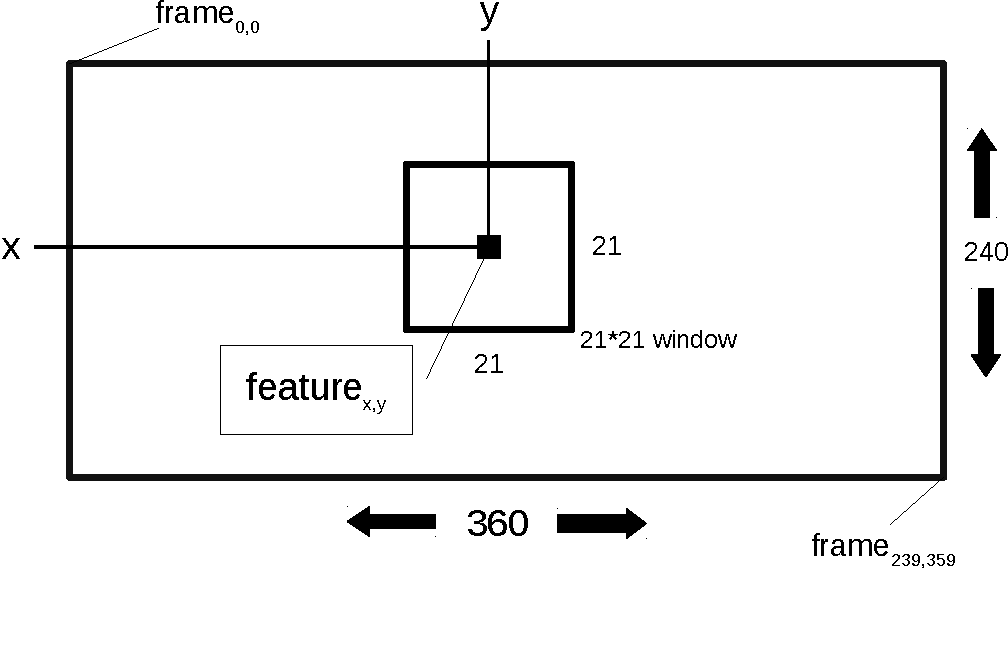
\includegraphics[width=0.8\textwidth]{frameWindow}
	\caption{Window arround feature within a frame}
	\label{frameWindowFig}
\end{figure}
\FloatBarrier


\subsection{First Frame Processing}

When \vc{} gets $firstFrame_{0,0}$, \file{int} $featuresArray[2][30]$ and $secondFrame_{0,0}$ he starts processing the first frame.

The goal is to get 4 values per \keyword{feature}:
\begin{itemize}
	\item $G_{XX}$ -- vertical gradient of the feature
	\item $G_{YY}$ -- horizontal gradient of the feature
	\item $G_{XY}$ -- cross gradient of the feature
	\item $det = \frac{1}{G_{XX}G_{YY}-G_{XY}G_{XX}}$
\end{itemize}

As shown in Figure~\ref{frameWindowFig}, we use a $21\times21$ \option{pixel window} around the feature:

$$G_{XX} = \sum_{i=1}^{21}\sum_{j=1}^{21} grad_{x}[i,j]^{2}$$
$$G_{YY} = \sum_{i=1}^{21}\sum_{j=1}^{21} grad_{y}[i,j]^{2}$$
$$G_{XY} = \sum_{i=1}^{21}\sum_{j=1}^{21} grad_{x}[i,j]\times grad_{y}[i,j]$$

Where, for a pixel element of the window -- $firstWindow_{i,j}$:
$$grad_{x}[i,j] = \frac{firstWindow_{i+1,j} - firstWindow_{i-1,j}}{2}$$
$$grad_{y}[i,j] = \frac{firstWindow_{i,j+1} - firstWindow_{i,j-1}}{2}$$


\subsection{Displacement computation}

\begin{figure}[!htbp]
\begin{algorithmic}
	\ForAll {$firstWindow_{i,j}$ and $secondWindow_{i,j}$}

	\State $diff\_frames = firstWindow_{i,j} - secondWindow_{i+d_{x},j+d_{y}}$

	\State $frames\_mismatch.x = diff\_frames\times grad_{x}[i,j]$
	\State $frames\_mismatch.y = diff\_frames\times grad_{y}[i,j]$

	\State $d_{x} = det\times (G_{YY}\times frames\_mismatch.x - G_{XY}\times frames\_mismatch.y)$
	\State $d_{y} = det\times (G_{XX}\times frames\_mismatch.y - G_{XY}\times frames\_mismatch.x)$

	\EndFor
\end{algorithmic}
\end{figure}

%----------------------------------------------------------------------------------------

\section{Implementation on \vc}

%----------------------------------------------------------------------------------------
